\subsection{Mecanismos básicos}
Para facilitar o entendimento dos processos descritos a seguir, a Figura \ref{fig:ring} representa a estrutura física de um anel de armazenamento.
	
\begin{figure}[!htb]
	\centering
	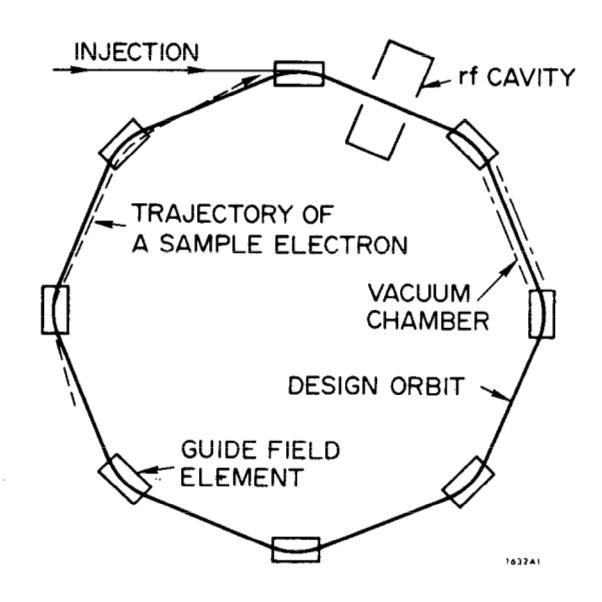
\includegraphics[width=0.6\linewidth]{./Figuras/fig1.jpeg}
	\caption{Diagrama esquemático de um anel de armazenamento de elétrons. Retirado de \cite{sands1970physics}.}
	\label{fig:ring}
\end{figure}
	
Um feixe de elétrons é injetado em uma câmara circular em vácuo. Campos magnetostáticos guiam as partículas pela câmara de vácuo. Tais campos são chamados de \emph{campos guia}. A interação eletromagnética entre o campo guia e os elétrons causa uma aceleração centrípeta do feixe, curvando assim sua trajetória e gerando um \emph{órbita fechada} desejada e desenhada a partir da escolha criteriosa do campo.
	
Esse campo guia, além de fechar a trajetória em uma órbita, tem propriedades focalizadoras que fazem com que cada elétron execute oscilações pseudo-harmônicas na transversal, as quais são chamadas de \emph{oscilações betatron}.
	
A cada volta, o elétron perde uma pequena parte da sua energia em forma de \emph{radiação síncrotron}. Esta energia perdida é reposta através de campos elétricos oscilantes no tempo gerados na \emph{cavidade de rádio frequência} (RF) e que aceleram longitudinalmente o feixe. Essas pequenas variações de perda e ganho da energia dos elétrons causam também oscilações no comprimento de órbita, no período de revolução, e ainda, no instante de chegada $\tau$ dos elétrons na cavidade de RF. As oscilações no plano energia-$\tau$ são chamadas de \emph{oscilações síncrotron} (ou oscilações de fase). Essas oscilações longitudinais dos elétrons são medidas em relação às \emph{partículas síncronas}, que são definidas como aqueles elétrons idealizados cujas energias, períodos de revolução e fase de chegada à cavidade de RF têm valores nominais.

Existem fases ideais de chegada à cavidade de RF em que o campo elétrico da cavidade é tal que a energia reposta por ele coincide com a energia média perdida pelos elétrons em cada volta. Cada uma destas fases ideais é chamada de \emph{fase síncrona}. O \emph{número harmônico} de um anel é definido como sendo a razão inteira entre a frequência de RF e a frequência de revolução dos elétrons. O número harmônico nos dá então o número de fases síncronas que podem ser acomodados no anel. Ao redor de cada uma destas fases síncronas, que são pontos fixos do espaço de fase energia-$tau$ nos quais se situam as partícula síncronas, pode-se ter uma distribuição de elétrons descrevendo oscilações síncrotron. Estas distribuições de elétrons em torno de das fases síncronas são chamadas de pacotes ou \emph{bunches}. Tipicamente o número harmônico dos anéis assume valor alto, permitindo assim um grande número de bunches e, em consequência, uma corrente de feixe circulante mais intensa.
	
A perda de energia por radiação síncrotron junto com a compensação gerada pela cavidade de RF causa um lento amortecimento da radiação de todas as amplitudes de oscilação, fazendo com que a trajetória de cada elétron tenda à trajetória do elétron de referência, o qual possui velocidade constante ao longo da órbita ideal.
	
Amortecimento da radiação não conserva o espaço de fase, então pode-se injetar vários \textit{bunches} no mesmo anel. O amortecimento de todas as amplitudes de oscilação é efetivamente preso devido à excitação contínua das oscilações por um "ruído" na energia do elétron, que vem do fato da radiação síncrona ser emitida em fótons de energia discreta. Este fenômeno é chamado de flutuação quântica da perda de energia. Em condições estacionárias, um equilíbrio é alcançado entre a excitação quântica e o amortecimento da radiação, levando a uma distribuição estatística estacionária das amplitudes e fases de oscilação dos elétrons em um \textit{bunch}. O \textit{bunch}, então, toma forma de uma tira elástica viajante, a qual tem tamanho e forma estacionários, com uma distribuição Gaussiana das amplitudes em cada coordenada transversal e longitudinal (Figura \ref{fig:fig2}). 
	
\begin{figure}[!htb]
	\centering
	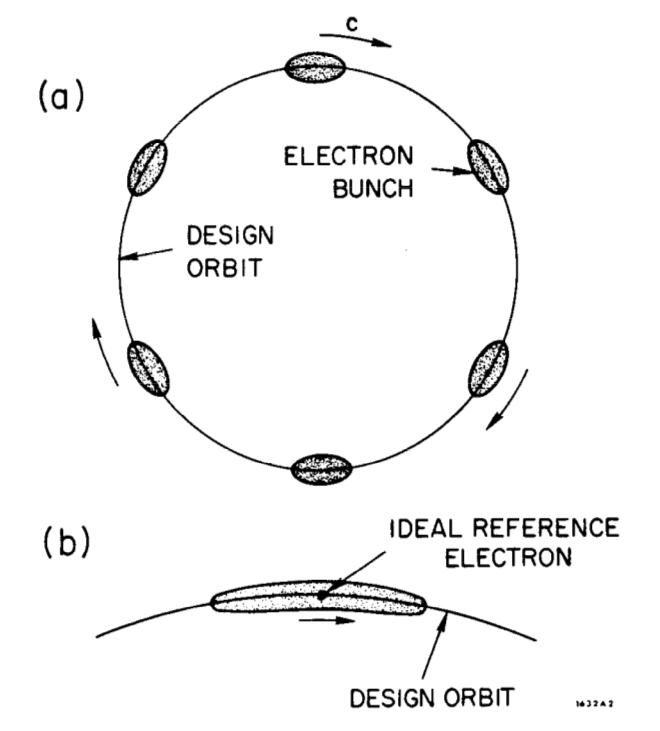
\includegraphics[width=0.55\linewidth]{./Figuras/fig2.jpeg}
	\caption{\textit{Bunches} circulando em um anel de armazenamento. Retirado de \cite{sands1970physics}.}
	\label{fig:fig2}
\end{figure}
	
Para cada coordenada do elétron, existe uma amplitude de oscilação máxima chamada de abertura dinâmica, a qual o elétron não fica mais preso dentro do \textit{bunch}. A abertura dinâmica para cada coordenada é definida por um obstáculo físico (tamanho da câmara de vácuo, por exemplo) ou por efeitos não-lineares nas forças focalizadoras, gerando trajetórias não-limitadas.